\documentclass[12pt]{article}
\author{Martin Ludvigsen}
\title{TMA4280 - Project 1}

\usepackage{amsmath}
\usepackage{graphicx}
\graphicspath{{figures/}}
\usepackage{subcaption}
%\usepackage{float}
\begin{document}
\maketitle
\section{Introduction}
The project was written in Fortran, using a home-brewed Makefile and Python for plotting. The organization of the folders
should make it obvious where the files are located. The project can be downloaded from github using this link:
\begin{equation*}
    \texttt{https://github.com/martilud/TMA4280project1.git}
\end{equation*}

The objective of the project is to calculate $\pi$ using two formulae, rewritten slightly from the problem description. First, the simple, yet beautiful Riemann-Zeta/Basel problem formula
first proved by Euler:
\begin{equation}
    \lim_{n \rightarrow \infty} \sum_{i = 1}^n \frac{1}{i^2} = \frac{\pi^2}{6},
    \label{eq:zeta}
\end{equation}
and secondly, the slightly more complex, "original" Machin formula, based on the Taylor series expansion of $\text{arctan} x$:
\begin{equation}
    \lim_{n \rightarrow \infty} \sum_{i = 1}^n (-1)^{i-1} \frac{1}{2i-1}\left(4 \left(\frac{1}{5}\right)^{2i-1} - \left(\frac{1}{239}\right)^{2i-1}\right) = \frac{\pi}{4}.
    \label{eq:mach}
\end{equation}
All of our experiments we're done on the supercomputer Idun, using $4$ nodes and $20$ tasks per node.

\section{Question 1. Serial Implementation}
In both formulae, we can expect roundoff errors for large $i$. In double precision, the mantissa uses $52$ bits, meaning the smallest "distance" we can measure
between numbers is $2^{-52} \approx 2.22 \times 10^{-16}$. This is also called the precision of double precision numbers.
Note this is not the same as the smallest number we can represent in double precision. We can actually represent numbers as small as
$\pm 2.23 \times 10^{-308}$, but when we start doing mathematical operations, we make round off errors. 
This also means that the order of operations in our calculations actually matter, as floating point operations are not commutative.
Note that for \eqref{eq:mach}, from now on called \texttt{mach},
it's much faster to calculate $\left(\frac{1}{5}\right)^{2i-1}$ by saving $\left(\frac{1}{5}\right)$ in a variable and multiplying it by 
$\left(\frac{1}{5}\right)^2$ each iteration instead of calculating it bottom up each iteration. We call this method "method 1", and calculating $\left(\frac{1}{5}\right)^{2i-1}$ bottom up
each iteration for "method 2".
My implementations showed to be sufficiently numerically stable, as we will see later. 

\section{Question 2. Unit Test(s)}
A unit test is a fast test of our program. The purpose of a 
unit test is to check the logic in our code to ensure it runs correctly.
In larger programs, one usually runs unit tests on small parts of code
to ensure that every part works as intended. In our toy example, we only
have to check if the program actually runs, and returns something slightly logical.
For this, I could have written a separate Fortran program, bash script of some sort or used some unit testing software.

But before we write anything, what whould we test to ensure our code works correctly? For \eqref{eq:zeta}, from now on called \texttt{zeta},
we see that a partial sum will always be (up to floating point errors), between $1$ and
$\frac{\pi^2}{6}$. Thus we can check if the error in our calculated $\pi_n$, calculated as $|\pi - \pi_n|$, is somewhere between $1$ and $\pi - \sqrt{6}$.

Using similar logic for \texttt{zeta},
we see that the first term in the sum is $\frac{4}{5} - \frac{1}{239}$, and all subsequences should be closer to $\pi$ than this by the error bound provided by the
alternating series test (REFERANSE). Thus, we can check if the error is larger than $4 \times(\frac{4}{5} - \frac{1}{239}) - \pi$, as no subsequence should have a higher error than this.  

When implementing, it proved to be simplest to just program the test into our original program, and use the command line to input if we want to test. This was mostly because bash scripts can't
handle floating point numbers and i did not want to bother linking different Fortran scripts together. The simplest solution is often the best solution.

We can then make a command in the Makefile to execute our unit test(s) easily, either by typing for example \texttt{make zeta0utest} to run the \texttt{zeta0} unit test or
\texttt{make utest} to run all unit tests. Figure \ref{fig:Q2} shows the output of our unit test(s). It works! 
\begin{figure}[!htb]
    \centering
    \caption{Result of running \texttt{make utest}}
    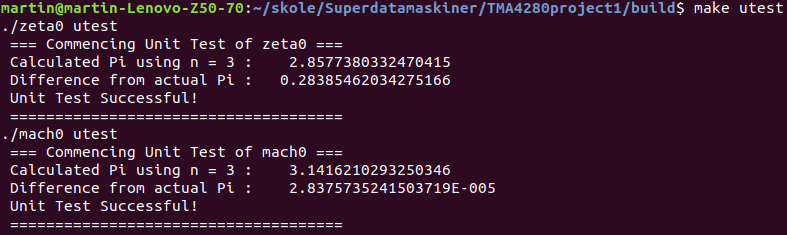
\includegraphics[width=\textwidth]{Screenshot2}
    \label{fig:Q2}
\end{figure}

\section{Question 3. Verification Test(s)}
Now that we know our programs work, we have to see if the mathematics behave nicely. For simplicity, this was also programmed directly into our existing program similarily to the Unit Test.
In our verification test, we check the error for many different $n$, and save the resulting error and the time it took calculate in a textfile. This can be executed similarily
to the unit test, just swap the word \texttt{utest} with \texttt{vtest}.

Results from running the verification tests are shown in figures \ref{fig:Convergence1} and \ref{fig:Time1}. 

\begin{figure}[!htb]
    \centering
    \caption{Convergence result of running \texttt{make vtest}}
    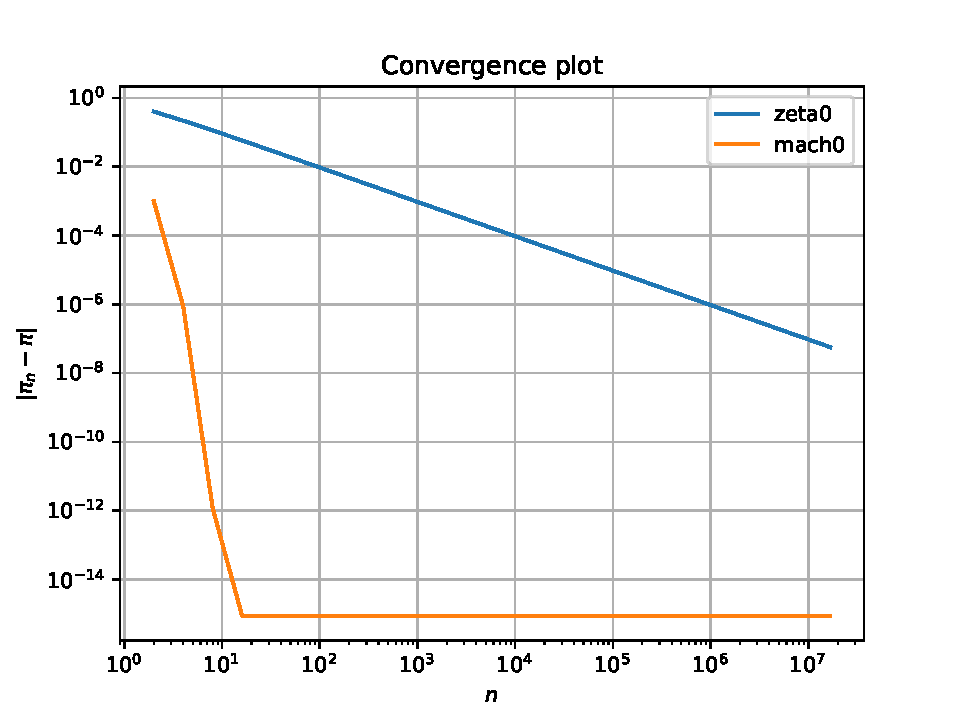
\includegraphics[width=\textwidth]{Convergence1}
    \label{fig:Convergence1}
\end{figure}

\begin{figure}[!htb]
    \centering
    \caption{Timing result of running \texttt{make vtest}}
    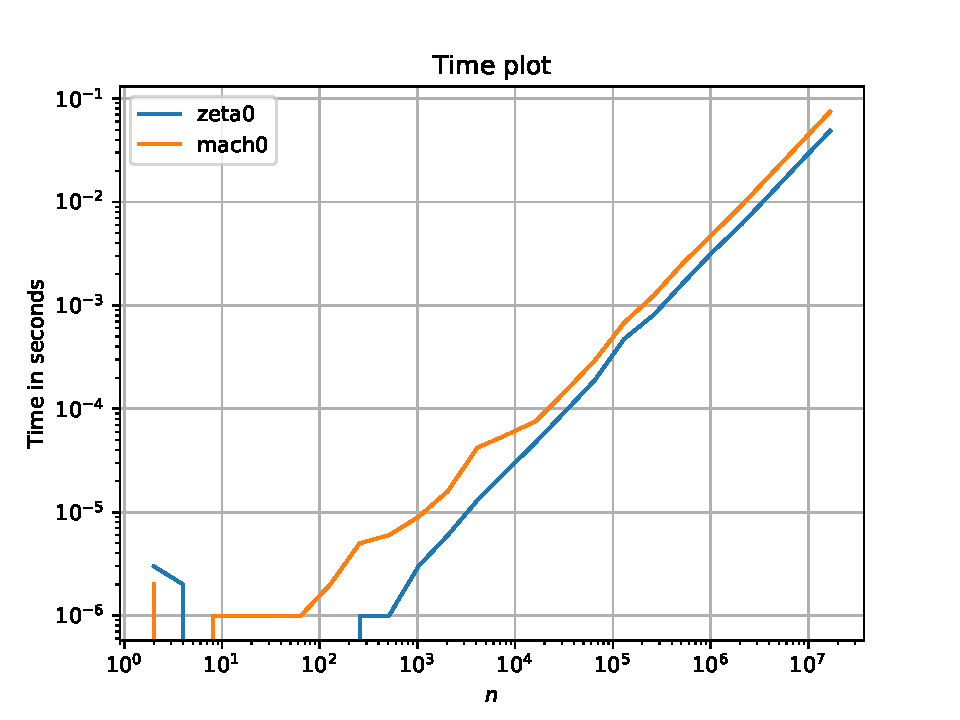
\includegraphics[width=\textwidth]{Time1}
    \label{fig:Time1}
\end{figure}
We see that the Machin formula quickly converges to a very low number, specifically $8.9 \times 10^{-16}$. 
This is obtained after only $16$ iterations, and subsequent iterations do not improve the accuracy of our estimate.
This is because of roundoff errors. Looking at \texttt{mach} we see that the sixteenth term is $\frac{1}{31}((2.15 \times 10^{-22}) + (1.86 \times 10^{-74}))$. 
As i mentioned earlier, this can be represented as a floating point number, but the computer is unable to evaluate the sum of the two numbers correctly.
It is also completely unable to evaluate the number we obtain when we add this very small term to our sum variable. Thus, we get "stuck" at an error of $8.9 \times 10^{-16}$.

For the Riemann-Zeta formula, the convergence is slow, and we are unable to reach a good estimate of $\pi$ even after $2^{24} \approx 1.68 \times 10^7$ iterations. Note that
the first term where we approach the precision available to us is when $\frac{1}{i^2} \approx 10^{-16}$, meaning the $10^8$th iteration. 

Looking at the time the different foruma uses, we see that the Machin formula is vastly superior here as well. Ironically, there are some round-off errors in timing for very few iterations as well.
This is somewhat surprising, as the Riemann-Zeta formula is so much simpler. Note that
using the other method for \texttt{mach} is more slower than \texttt{zeta}, and we will have to use it later.

\section{Question 4. Data distribution}
Now onto some distributed parallell computing. This means that we have different processing units with their own memory, and we have to use a Message Passing Interface (MPI) to transfer
data between processes.
In our program, we have one process calculate each term of the sum, save it into a vector, distribute the vector to different processes and have each process calculate
their partial sums, before adding the partial sums together. This is a bad decision, because there is an obvious bottleneck. One of the main problems with high performance computing
are the different bottlenecks. Here, the bottleneck is that one process has to do a lot of work serially. Even worse, the amount of work that has to be done serially perfectly scales
with the workload. Amdahl's law then predicts an upper limit to the speedup we can achieve. The theoretical speedup can be written as
\begin{equation}
    S(s) = \frac{1}{(1-p) + p/s}
\end{equation}
where $s$ is the speedup achieved by the part of the program that is parallellizable, which is often assumed to be equal to the number of processing units, and $p$ is the portion of the 
program that has to be done serially. The point is that $S \le \frac{1}{1-p}$, meaning that if a large part of our program has to be done serially, we can only achieve a marginal speedup.

The solution would be to ensure that as much of the program as possible is done in parallell. This can be done by having each process calculate the terms in their partial sum, not saving it
in a vector and adding the terms before summing the different partial sums to the master process. Here, the only serial parts of the program is taking arguments from the command line
and the overhead from MPI. I guess the reason we don't do this is that our program is a good example of data-parallellism that MPI is most often used for.

I actually made a unit test for this part of the program as well, which splits the data using \texttt{MPI\_Scatter}, checks if the resulting subvectors match the original vector, 
which is transferred using \texttt{MPI\_Bcast}, and uses
\texttt{MPI\_Reduce} to check if any process had any erroneous data.

\section{Question 5 \& 6. MPI Implementation}
We've already mentioned how the resulting program works, and we also use \texttt{MPI\_Reduce} here for the final summation of the different
partial sims. In addition we have to use \texttt{MPI\_Init}, 
\texttt{MPI\_Comm\_size}, \texttt{MPI\_Comm\_rank} and \texttt{MPI\_Finalize}, as we can't really do anything in MPI without invoking these. 
Most MPI programs can be made using the mentioned functions and \texttt{MPI\_Send} and \texttt{MPI\_Recv} (we did not need these as \texttt{MPI\_Scatter} was more convenient),
but there are virtually no limits to how fancy you can make your MPI program
by using more advanced MPI functions.

A unit test was implemented similarily to the single-process program.

For timing we use the \texttt{MPI\_Wtime} function. Note there is a big pitfall here. Firstly, there is a large difference between CPU clock time
and wall time. CPU time measures the amount of clock cycles on the CPU (which only makes sense in the context of what CPU you are using),
while wall time is the time used in seconds. The default Fortran function for measuring time, \texttt{CPU\_TIME} measures clock time, but it also sums the time used by different
processes on the CPU. In other words, it is mostly useless for measuring the speed of parallel programs. For all timings, i only timed the parts of the code including actual computations,
ignoring I/O and initilization of MPI. 

Convergence results are shown in figure \ref{fig:Convergence2},
and timing results are shown in figure \ref{fig:Time2}.
\begin{figure}
    \centering
    \begin{subfigure}[!htb]{0.45\textwidth}
        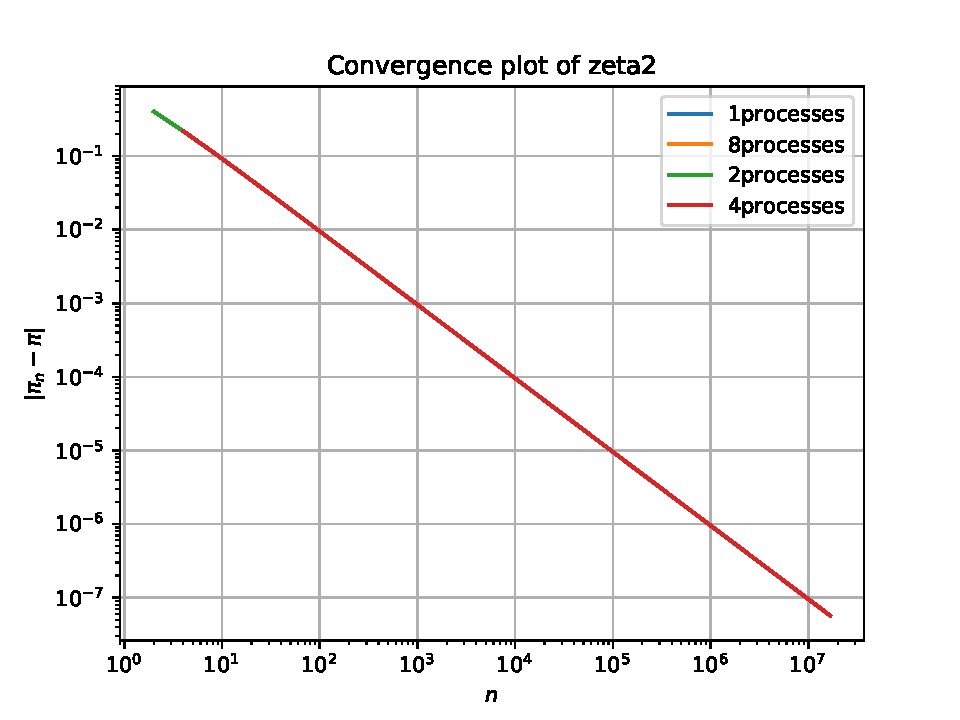
\includegraphics[width=\textwidth]{zeta2Convergence}
    \end{subfigure}
    \begin{subfigure}[!htb]{0.45\textwidth}
        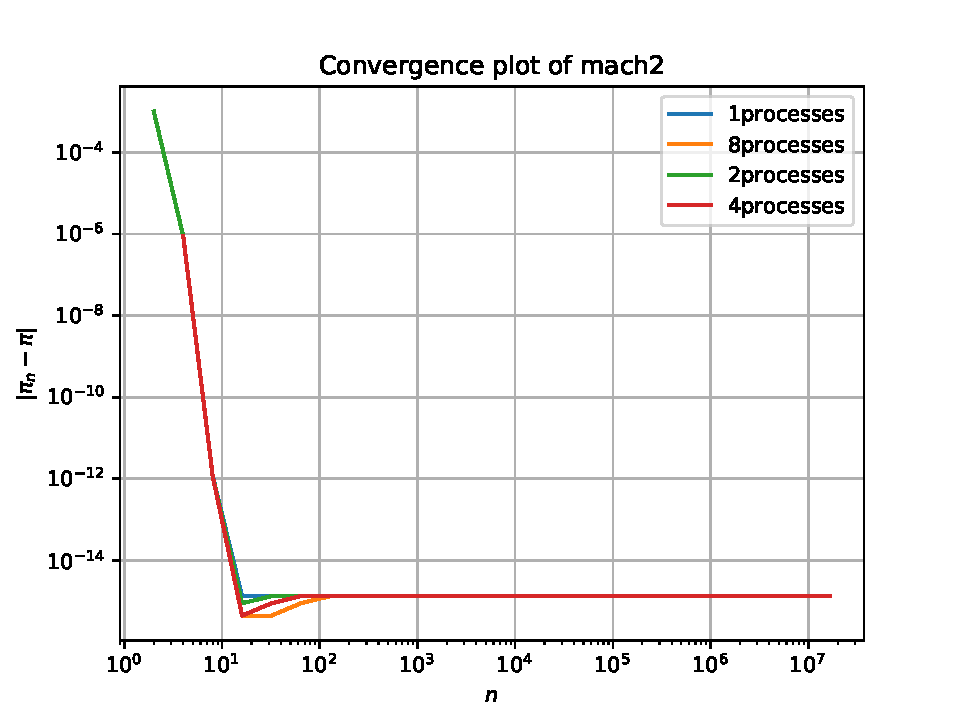
\includegraphics[width=\textwidth]{mach2Convergence}
    \end{subfigure}
    \caption{Convergence of our MPI programs}\label{fig:Convergence2}
\end{figure}
\begin{figure}
    \centering
    \begin{subfigure}[!htb]{0.45\textwidth}
        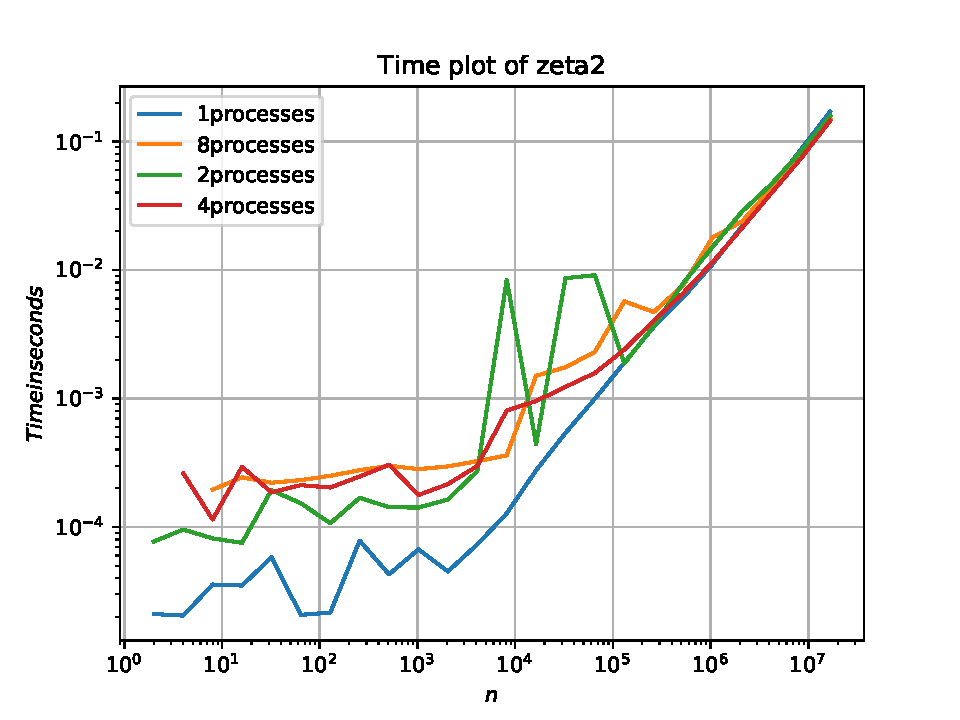
\includegraphics[width=\textwidth]{zeta2Time}
    \end{subfigure}
    \begin{subfigure}[!htb]{0.45\textwidth}
        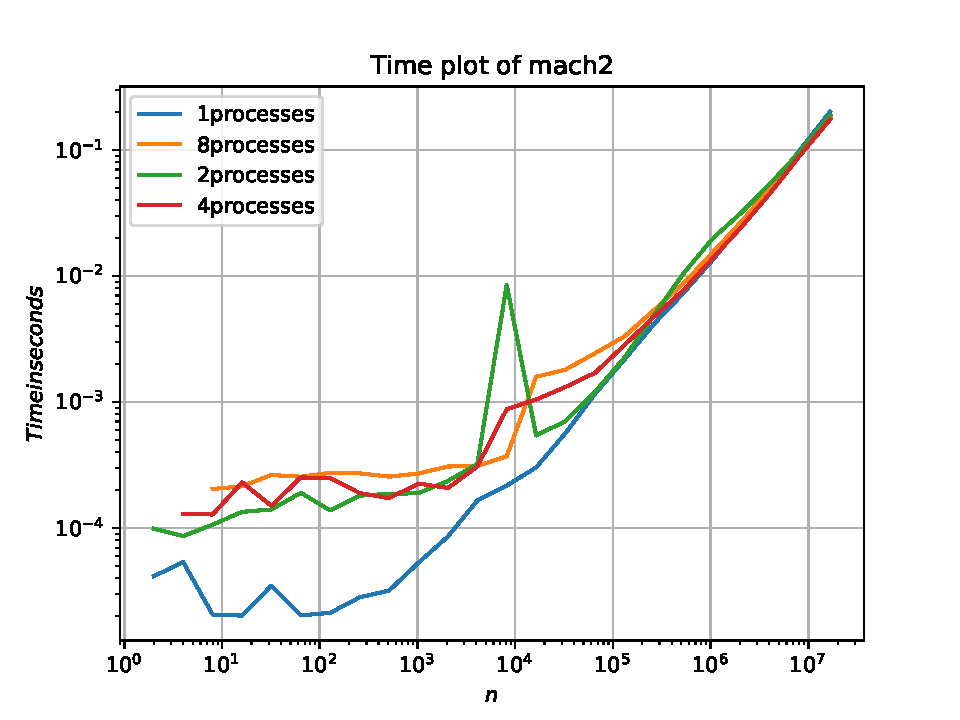
\includegraphics[width=\textwidth]{mach2Time}
    \end{subfigure}
    \caption{Timing of our MPI programs}\label{fig:Time2}
\end{figure}

For convergence we see similar trends to the single-process program. However, for \texttt{mach} we see that the error slightly differs for different amount of processes.
For \texttt{zeta}, there is also a slight difference in error, although nearly invisible. This is because floating point arithmetic does not comute. 
For floating point numbers $a$ and $b$, we have that $a + b \neq b + a$ (again, noncommutative),
because of the issues with precision we discussed earlier. When we use MPI, we slightly switch the order
of our arithmetic operations, meaning we end up with slightly different answers (although approximately the same) every time. The difference in error for $p=2$ processes and $p=8$ is still
marginally small, on the order of $10^{-16}$, which is the precision we can expect. Also note that the single-process program and our MPI program converges to slightly different numbers, the MPI 
implementation doing a bit worse.

Before discussing timing, we need to take a slight intermission. We've already noted that computers seem to behave non-deterministically. Well, computers are deterministic,
but modern computers are extremely complex, from the hardware they are built from to the software they run on. The specifics of computer hardware is kept secret by vendors, 
adding another layer of complexity. This means that computers, at some level, behave randomly. We have to measure the time a program uses to run because we cannot determine it a priori.

Why does this matter? There will always be some random noise in timing data, but we see a clear trend. As predicted, MPI actually worsens the performance for low $n$, as the overhead
caused by MPI simply is not worth it. For large $n$ we see a slight speedup the more MPI processes we have.

\section{Question 7. OpenMP implementation}
We've looked at distributed memory systems, now we'll look at shared memory systems. This means that we split the work into several threads executing on the same node (same CPU) with the same memory.
This is done easily using OpenMP, as we simply have to wrap the critical parts of our loops (where most of the work is done) in \texttt{\$!OMP PARALLELL DO}. If the compilator understands what
this means, it will do its best in parallellizing the code for us. There exists more fancy ways of using OpenMP, but for now this is all we need. A problem on shared memory systems are race 
conditions.
This means that several threads are "competing" over the same memory, and the changes done by one thread is overwritten by another. To avoid this, we add a \texttt{REDUCTION} clause which
executes a reduction similar to MPI.

Another huge problem with OpenMP is that we can no longer have loops where the there are dependencies between different iterations. This means our faster method of calculating
\texttt{mach} has to be thrown out the window for the parallellization to work.

A unit test was implemented similarily to the single-process program.

For timing, we use \texttt{omp\_get\_wtime}, noting the problems with timing from earlier.

For the OpenMP implementation, I did not make a vector and divide this, but paralellized \texttt{zeta0} and \texttt{mach0} instead. In the next question we will use OpenMP to parallelize 
creating a vector and distributing it between MPI processes. Convergenc results are shown in figure \ref{fig:Convergence3} and timing results are shown in figure \ref{fig:Time3}.
\begin{figure}
    \centering
    \begin{subfigure}[!htb]{0.45\textwidth}
        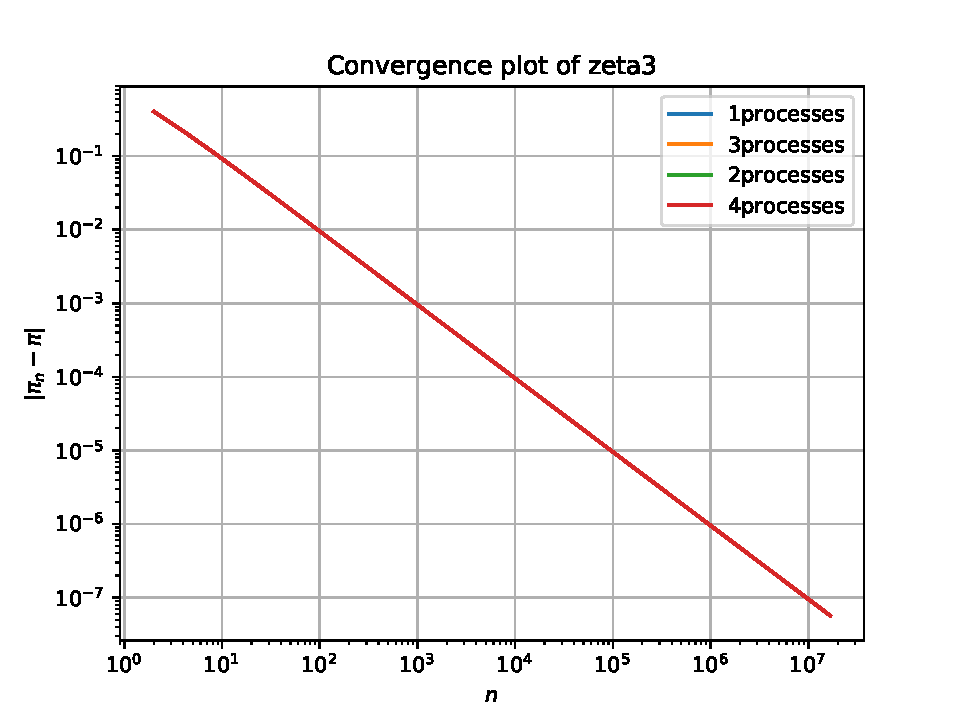
\includegraphics[width=\textwidth]{zeta3Convergence}
    \end{subfigure}
    \begin{subfigure}[!htb]{0.45\textwidth}
        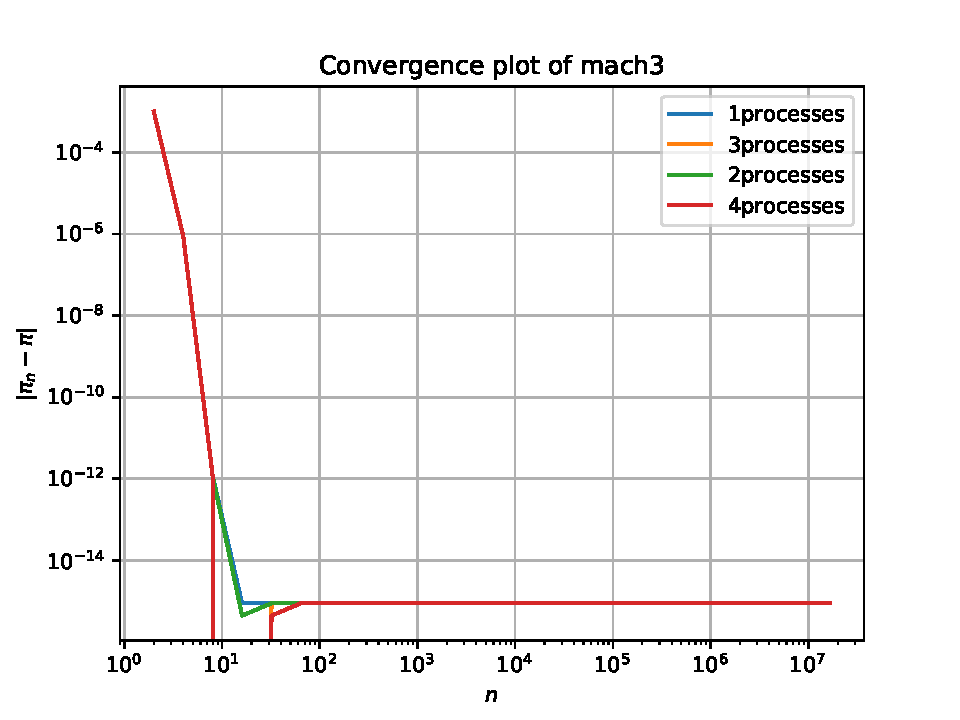
\includegraphics[width=\textwidth]{mach3Convergence}
    \end{subfigure}
    \caption{Convergence of our OpenMP programs}\label{fig:Convergence3}
\end{figure}
\begin{figure}
    \centering
    \begin{subfigure}[!htb]{0.45\textwidth}
        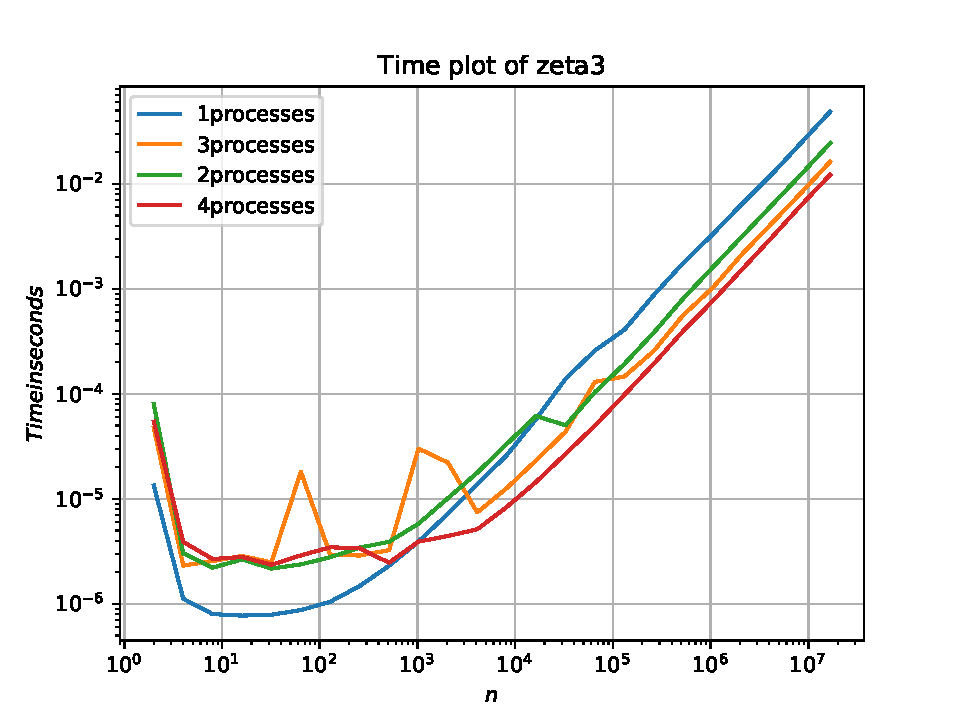
\includegraphics[width=\textwidth]{zeta3Time}
    \end{subfigure}
    \begin{subfigure}[!htb]{0.45\textwidth}
        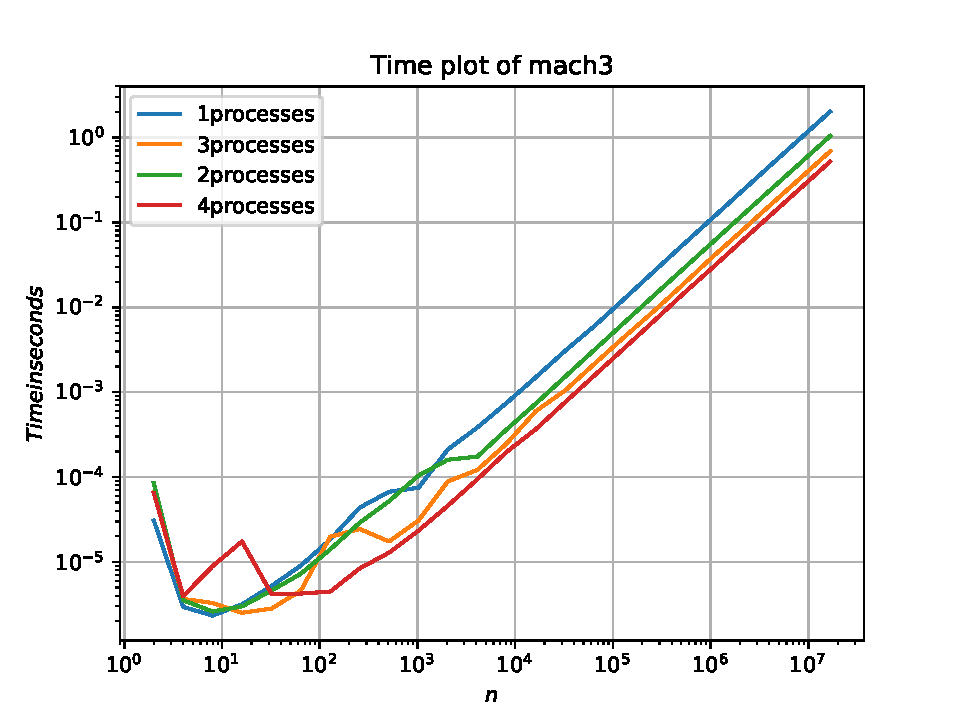
\includegraphics[width=\textwidth]{mach3Time}
    \end{subfigure}
    \caption{Timing of our OpenMP programs}\label{fig:Time3}
\end{figure}
The convergence results are almost identical to the MPI implementation, but now the answer converges to the same result as the single-threaded version of our program.
We do see that we get different results from different number of threads, again noting that floating point opperations do not commute.
For the timing, we actually see a clear speedup. Here, we parallellized all paralellizable parts of the program, so we expected such. For high $n$, the speedup approaches the number of
processes, which is about the best speedup we can hope to achieve. For low $n$, we again see that the overhead caused by OpenMP damages the speed of our program.

\section{Question 8. Hybrid MPI/OpenMP implementation}
Similarily to how we "simply" parallellized our single-proccess program using OpenMP, we can now parallellize our MPI program using OpenMP. Thus we can get the best of both worlds.
We can divide the work between different processes (which corresponds to different nodes on Idun) and each process divides the work into different threads 
(which correspond to cores on each node on Idun). This is great, although it adds another layer of things that can go wrong. 

A unit test was implemented similarily to the single-process program. In addition, it prints the MPI rank and the OpenMP thread number to ensure they are working as intended.

Convergence for this method is very similar to the last
implementations, so i won't bother showing it. Timing results are shown in figure \ref{fig:Time4}.
\begin{figure}
    \centering
    \begin{subfigure}[!htb]{0.45\textwidth}
        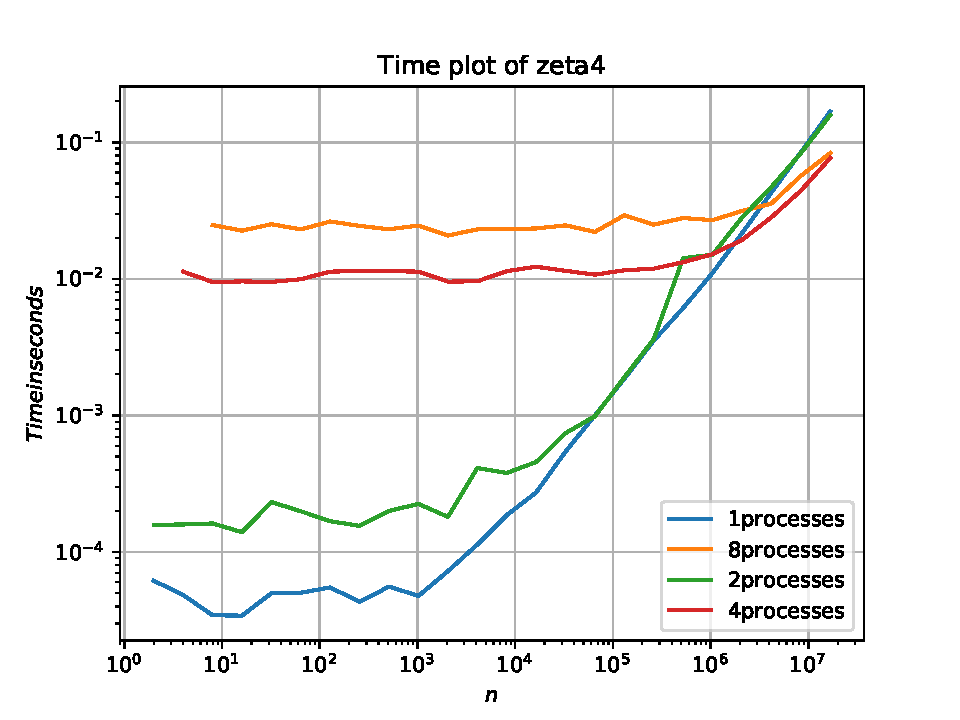
\includegraphics[width=\textwidth]{zeta4Time}
    \end{subfigure}
    \begin{subfigure}[!htb]{0.45\textwidth}
        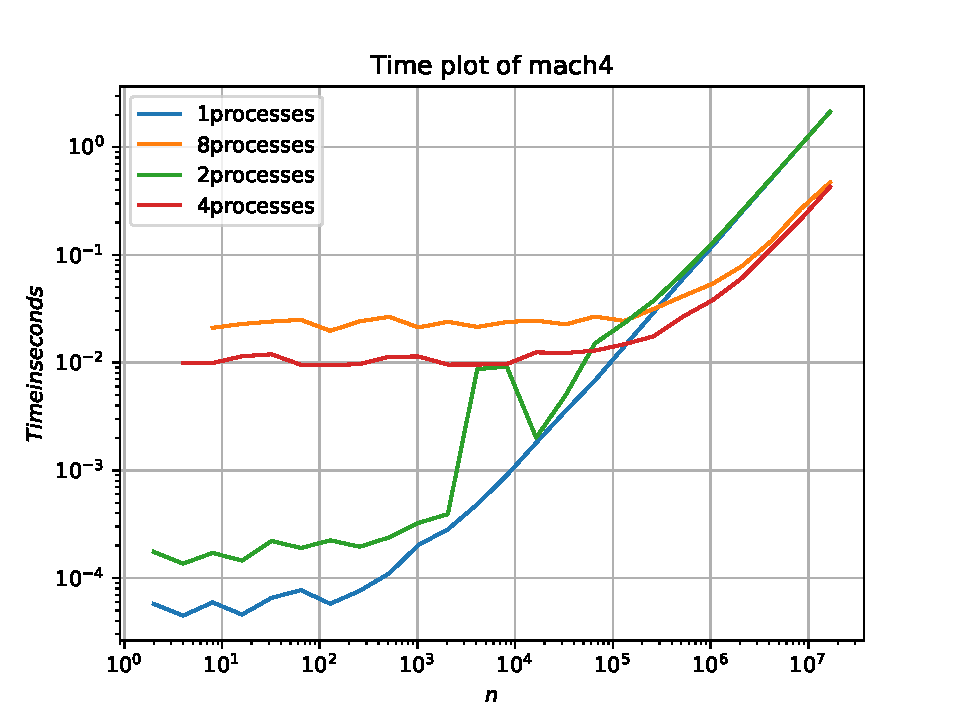
\includegraphics[width=\textwidth]{mach4Time}
    \end{subfigure}
    \caption{Timing of our hybrid MPI/OpenMP programs}\label{fig:Time4}
\end{figure}
The timings are actually very interesting. In these plots, the number of processes refers to the number of MPI processes. I let OpenMP decide how many threads to use. 

\section{Question 9. Discussion}

We can easily calculate the \textbf{amount} of memory used by the the single-process program. 
We will only look at the calculation part, ignoring I/O. We will also only look at what is stored, ignoring
the memory used by other functions or arithmetic operations.
\texttt{zeta0} needs to store two integers and a float, which each need $8$ bytes. \texttt{mach0} uses two integers and five or seven floats, depending on how it is implemented. Thus \texttt{mach0}
uses more memory, but the amount of memory is so tiny it's insignificant. Note that the amount of memory is not dependent on $n$, meaning the memory is $O(1)$.

For the MPI version of the program, we need to store an additional $n$ floats in the vector, and each process nees a copy of this vector. Thus the memory requirement is $O(np)$, where $p$
in number of processes. This is not good, as memory requirements could become problematic.

For the OpenMPI version of the program, we only have to store the vector once, but there is probably some memory that scales with number of threads. For the reduction the different threads
probably needs a seperate variable for their partial sum and loop variables. Thus the memory requirement is $O(n+p)$, assuming the memory requirement scales linearly with number of threads.  
We probably have $n >> p$, meaning the memory requirement is realistically $O(n)$. The results are summarized in table \ref{tab:memory}.
\begin{table}[]
\begin{tabular}{llll}
& Single-process & MPI & OpenMP \\
    Memory requirement & $O(1)$ & $O(np)$ & $O(n + p)$ 
\end{tabular}
    \caption{Memory requirements for the different programs}
    \label{tab:memory}
\end{table}

For \textbf{generating the vector} we can simply count the number of operations. First note that FLOPS do not directly correspond to the time used. 
For example, addition usually takes less clock cycles
than division or finding a square root, although this is often hidden in a web of pipelining and multiple issue, not to mention caching.
The point is that FLOPS do not directly correspond to "amount of useful work done" and is therefore a somewhat pointless exercise. However, it is also useful as a coarse indicator of performace.
We will count all floating-point operations as a FLOP, and ignore the cost of integer operations. 
For \texttt{zeta}, each terms consist of dividing by a number squared, which corresponds to $3$ FLOPS. 
Thus, we need $3n$ operations to produce the vector. For \texttt{mach}, the amount of FLOPs depends on the method used. 
Using method 1 (not calculating $x^{(2i-1)}$ explicitly each time), we have to do around $11$ FLOPs every iteration, depending on how you count. We then end up with $11n$ FLOPs to produce the vector.
If we calculate $x^{2i-1}$ explicitly each time and assume that it takes $2i-2$ FLOPs to calculate $x^{2i-1}$ (because $x^{2i-1} = x \times x ... \times x$ means $2i-1$ multiplications) we end up
with $7 + 2i - 2$ FLOPs per term. The total amount of FLOPs needed to produce the vector is then $4n + n^2$. Note this scales a lot worse with the problem size, so hopefulley exponentiation is
implemented in a more clever way so we avoid this bad scaling.

When the vector is made, \textbf{calculating the sum} just requires us to add all the elements of the vector, which is $n-1$ FLOPs. For the multiprocessor programs, the amount of FLOPs is the same.
Each process has to do $n/p - 1$ FLOPs, and adding the partial sums together requires another $p-1$ FLOPs: $(n/p - 1)\times p + p-1 = n-1$.

\textbf{Load balance} is a way of describing if the amount of work each process does is the same. In the parallell part of the program, we have "perfect" load balance as all processes have to add
the same amount of floating point numbers together. Load balance can become a problem if we have a loop where the contents of the loop vary from iteration to iteration. In OpenMP, we can use
different scheduling techniques to avoid this. However, the program as a whole is not load balanced, as one process has to do a lot of work before it shares the load with the other processes.         

How do we improve these properties? One way is to always use the fast way of calculating \texttt{mach}. Secondly, we want to avoid having one process calculate a vector and then distributing it.
It would be a lot more logical to just have each process calculate a partial sum and then add these together (which is basically how we did the OpenMP implementation).
This will also drastically reduce the memory requirements. When that is said, we can't really use less FLOPs, unless we abort the loop when we've reached a certain accuracy.

\section{Question 10. Conclusion}
Is this problem good for parallel processing? Yes and no. No because the problem simply is not large enough. The time used parallelizing the code vastly excedes the time the program uses to run.
Parallel processing should be used for critical, time-consuming calculations, where the overhead of MPI or OpenMP, in addition to the time spent programming it is actually worth it.
This problem is neither, and is only meant as a toy example of making parallel programs. When that is said, the problem is very easily parallellizable.
The proccess of making parallel programs usually does not start with making a single-process parallel program and then parallelizing it, but rather making a parallel alogorithm from the start.
Our problem is "embarassingly parallel", meaning that we can divide the work very easily. In that sense, it is very easy to just write two lines of code in OpenMP and get a speedup of the amount
of cores on your CPU(s). In that sense, parallel processing is attractive for this problem. When that is said, the fastest method for calculating $\pi$ to sufficient precision
was acutally our single-process \texttt{mach} program, but it would have probably been faster to use OpenMP if we had used more threads. 

Conclusion: Parallel programming is not easy, and should only be used on very large problems. Our problem is too small for parallel programming to be worth the effort,
but it was a useful exercise.

\section{Post-reflection}
\textbf{This section is probably not of interest to whoever is reading this, and is mostly a note to myself on where i made mistakes and what to look out for in the future}.

This project started off as fun and interesting. It ended up being very frustrating and time-consuming. I am very glad i've already taken a course on Parallell computations,
but this project has made me realize how much of the dirtywork we skipped in that class. List of frustrating things:
\begin{itemize}
    \item 1. Makefiles. They were a lot more work than i thought, and i am not satisfied with how my Makefile ended up.
    \item 2. Compilers. Compilers are both beautiful and very hard to work with. Specifically i had a lot of trouble getting my programs
        to interpret things with double precision when combined with MPI. I did a lot of useless experimentation here until things worked out.
    \item 3. Idun. Using Idun actually is not that hard, but it was somewhat more iffy than i thought. I especially had some problems making the compilers that worked
        on my computer work on Idun.
    \item 4. Bash scripts. Bash scripts are like ancient magic, and trying to write them is like delving into some old long forgotten art.
        I don't think i will every understand how to write them efficiently.
\end{itemize}
When that is said, these are the things that i wanted to learn from this subject, so it's stupid to complain. However, i wish this project would not have taken as much time as it did.
The "programming" part of the project took me maybe $2$-$3$ hours, but i have spent several tens of hours messing with the frustrating things mentioned earlier. I do however think 
that this was a useful project, and i feel much more familiar with supercomputing, and all of it's components, after this project.

\end{document}
